\documentclass[a4paper,twoside]{article}
% My LaTeX preamble file - by Nathaniel Dene Hoffman
% Credit for much of this goes to Olivier Pieters (https://olivierpieters.be/tags/latex)
% and Gilles Castel (https://castel.dev)
% There are still some things to be done:
% 1. Update math commands using mathtools package (remove ddfrac command and just override)
% 2. Maybe abbreviate \imath somehow?
% 3. Possibly format for margin notes and set new margin sizes
% First, some encoding packages and useful formatting
%--------------------------------------------------------------------------------------------
\usepackage{import}
\usepackage{pdfpages}
\usepackage{transparent}
\usepackage[l2tabu,orthodox]{nag}   % force newer (and safer) LaTeX commands
\usepackage[utf8]{inputenc}         % set character set to support some UTF-8
                                    %   (unicode). Do NOT use this with
                                    %   XeTeX/LuaTeX!
\usepackage[T1]{fontenc}
\usepackage[english]{babel}         % multi-language support
\usepackage{sectsty}                % allow redefinition of section command formatting
\usepackage{tabularx}               % more table options
\usepackage{booktabs}
\usepackage{titling}                % allow redefinition of title formatting
\usepackage{imakeidx}               % create and index of words
\usepackage{xcolor}                 % more colour options
\usepackage{enumitem}               % more list formatting options
\usepackage{tocloft}                % redefine table of contents, new list like objects
\usepackage{subfiles}               % allow for multifile documents

% Next, let's deal with the whitespaces and margins
%--------------------------------------------------------------------------------------------
\usepackage[centering,margin=1in]{geometry}
\setlength{\parindent}{0cm}
\setlength{\parskip}{2ex plus 0.5ex minus 0.2ex} % whitespace between paragraphs

% Redefine \maketitle command with nicer formatting
%--------------------------------------------------------------------------------------------
\pretitle{
  \begin{flushright}         % align text to right
    \fontsize{40}{60}        % set font size and whitespace
    \usefont{OT1}{phv}{b}{n} % change the font to bold (b), normally shaped (n)
                             %   Helvetica (phv)
    \selectfont              % force LaTeX to search for metric in its mapping
                             %   corresponding to the above font size definition
}
\posttitle{
  \par                       % end paragraph
  \end{flushright}           % end right align
  \vskip 0.5em               % add vertical spacing of 0.5em
}
\preauthor{
  \begin{flushright}
    \large                   % font size
    \lineskip 0.5em          % inter line spacing
    \usefont{OT1}{phv}{m}{n}
}
\postauthor{
  \par
  \end{flushright}
}
\predate{
  \begin{flushright}
  \large
  \lineskip 0.5em
  \usefont{OT1}{phv}{m}{n}
}
\postdate{
  \par
  \end{flushright}
}

% Mathematics Packages
\usepackage[Gray,squaren,thinqspace,cdot]{SIunits}      % elegant units
\usepackage{amsmath}                                    % extensive math options
\usepackage{amsfonts}                                   % special math fonts
\usepackage{mathtools}                                  % useful formatting commands
\usepackage{amsthm}                                     % useful commands for building theorem environments
\usepackage{amssymb}                                    % lots of special math symbols
\usepackage{mathrsfs}                                   % fancy scripts letters
\usepackage{cancel}                                     % cancel lines in math
\usepackage{esint}                                      % fancy integral symbols
\usepackage{relsize}                                    % make math things bigger or smaller
%\usepackage{bm}                                         % bold math!
\usepackage{slashed}

\newcommand\ddfrac[2]{\frac{\displaystyle #1}{\displaystyle #2}}    % elegant fraction formatting
\allowdisplaybreaks[1]                                              % allow align environments to break on pages

% Ensure numbering is section-specific
%--------------------------------------------------------------------------------------------
\numberwithin{equation}{section}
\numberwithin{figure}{section}
\numberwithin{table}{section}

% Citations, references, and annotations
%--------------------------------------------------------------------------------------------
\usepackage[small,bf,hang]{caption}        % captions
\usepackage{subcaption}                    % adds subfigure & subcaption
\usepackage{sidecap}                       % adds side captions
\usepackage{hyperref}                      % add hyperlinks to references
\usepackage[noabbrev,nameinlink]{cleveref} % better references than default \ref
\usepackage{autonum}                       % only number referenced equations
\usepackage{url}                           % urls
\usepackage{cite}                          % well formed numeric citations
% format hyperlinks
\colorlet{linkcolour}{black}
\colorlet{urlcolour}{blue}
\hypersetup{colorlinks=true,
            linkcolor=linkcolour,
            citecolor=linkcolour,
            urlcolor=urlcolour}

% Plotting and Figures
%--------------------------------------------------------------------------------------------
\usepackage{tikz}          % advanced vector graphics
\usepackage{pgfplots}      % data plotting
\usepackage{pgfplotstable} % table plotting
\usepackage{placeins}      % display floats in correct sections
\usepackage{graphicx}      % include external graphics
\usepackage{longtable}     % process long tables

% use most recent version of pgfplots
\pgfplotsset{compat=newest}

% Misc.
%--------------------------------------------------------------------------------------------
\usepackage{todonotes}  % add to do notes
\usepackage{epstopdf}   % process eps-images
\usepackage{float}      % floats
\usepackage{stmaryrd}   % some more nice symbols
\usepackage{emptypage}  % suppress page numbers on empty pages
\usepackage{multicol}   % use this for creating pages with multiple columns
\usepackage{etoolbox}   % adds tags for environment endings
\usepackage{tcolorbox}  % pretty colored boxes!


% Custom Commands
%--------------------------------------------------------------------------------------------
\newcommand\hr{\noindent\rule[0.5ex]{\linewidth}{0.5pt}}                % horizontal line
\newcommand\N{\ensuremath{\mathbb{N}}}                                  % blackboard set characters
\newcommand\R{\ensuremath{\mathbb{R}}}
\newcommand\Z{\ensuremath{\mathbb{Z}}}
\newcommand\Q{\ensuremath{\mathbb{Q}}}
%\newcommand\C{\ensuremath{\mathbb{C}}}
\renewcommand{\arraystretch}{1.2}                                       % More space between table rows (could be 1.3)
\newcommand{\Cov}{\mathrm{Cov}}
\newcommand\D{\mathrm{D}}
\newcommand*{\dbar}{\ensuremath{\text{\dj}}}

\newcommand{\incfig}[2][1]{%
    \def\svgwidth{#1\columnwidth}
    \import{./figures/}{#2.pdf_tex}
}

% Custom Environments
%--------------------------------------------------------------------------------------------
\newcommand{\lecture}[3]{\hr\\{\centering{\large\textsc{Lecture #1: #3}}\\#2\\}\hr\markboth{Lecture #1: #3}{\rightmark}}   % command to title lectures
\usepackage{mdframed}
\theoremstyle{plain}
\newmdtheoremenv[nobreak]{theorem}{Theorem}[section]
\newtheorem{corollary}{Corollary}[theorem]
\newtheorem{lemma}[theorem]{Lemma}
\theoremstyle{definition}
\newtheorem*{ex}{Example}
\newmdtheoremenv[nobreak]{definition}{Definition}[section]
\theoremstyle{remark}
\newtheorem*{remark}{Remark}
\newtheorem*{claim}{Claim}
\AtEndEnvironment{ex}{\null\hfill$\diamond$}%
% Note: A proof environment is already provided in the amsthm package
\tcbuselibrary{breakable}
\newenvironment{note}[1]{\begin{tcolorbox}[
    arc=0mm,
    colback=white,
    colframe=white!60!black,
    title=#1,
    fonttitle=\sffamily,
    breakable
]}{\end{tcolorbox}}
\newenvironment{problem}{\begin{tcolorbox}[
    arc=0mm,
    breakable,
    colback=white,
    colframe=black
]}{\end{tcolorbox}}

% Header and Footer
%--------------------------------------------------------------------------------------------
% set header and footer
\usepackage{fancyhdr}                       % header and footer
\pagestyle{fancy}                           % use package
\fancyhf{}
\fancyhead[LE,RO]{\textsl{\rightmark}}      % E for even (left pages), O for odd (right pages)
\fancyfoot[LE,RO]{\thepage}
\fancyfoot[LO,RE]{\textsl{\leftmark}}
\setlength{\headheight}{15pt}


% Physics
%--------------------------------------------------------------------------------------------
\usepackage[arrowdel]{physics}      % all the usual useful physics commands
\usepackage{feyn}                   % for drawing Feynman diagrams
%\usepackage{bohr}                   % for drawing Bohr diagrams
%\usepackage{tikz-feynman}
\usepackage{elements}               % for quickly referencing information of various elements
\usepackage{tensor}                 % for writing tensors and chemical symbols

% Finishing touches
%--------------------------------------------------------------------------------------------
\author{Nathaniel D. Hoffman}

\title{33-765 Midterm Exam}
\date{\today}
\begin{document}
\maketitle
\begin{quote}
    I hereby confirm that I have not collaborated with anybody else during completion of this exam, and I have not used external help that had been expressly excluded by the lecturer.
\end{quote}

\section*{1. Drawing Random Numbers from any Prescribed Probability Density}
Let $ p(x) $ be a probability density on the real numbers, and define its \textit{cumulative distribution function} $ Q(x) := \int_{- \infty}^x \dd{x'} p(x') $.
\begin{itemize}
    \item[1.] As a warm-up: Illustrate this definition by drawing some generic (and, pro-tip, not to singular) $ p(x) $ of your choice, as well as its associated $ Q(x) $ in the same diagram. Pay special attention to the values that $ Q(x) $ ultimately takes.

        Note: Don't just produce the plots; explain the relation between $ p(x) $ and $ Q(x) $ in the context of what will matter below.
        \begin{problem}
            See \Cref{fig:problem_1_plot} for the drawing. Note that $ Q(x) $ must begin at $ Q(- \infty) \equiv 0 $ (we're assuming the distribution is defined for negative $ x $), I drew one which was basically $ 0 $ for $ x < 0 $, so $ Q(0) \approx 0 $. Secondly, $ Q(\infty) \equiv 1 $ since $ Q(1) \equiv \int_{- \infty}^{\infty} \dd{x'} p(x') = 1 $ by normalization. Finally, in my plot, I attempted to show a bimodal distribution. The peaks and valleys should correspond to inflection points in the CDF, and the entire CDF should be monotonically increasing.
        \end{problem}
        \begin{figure}[h]
            \centering
            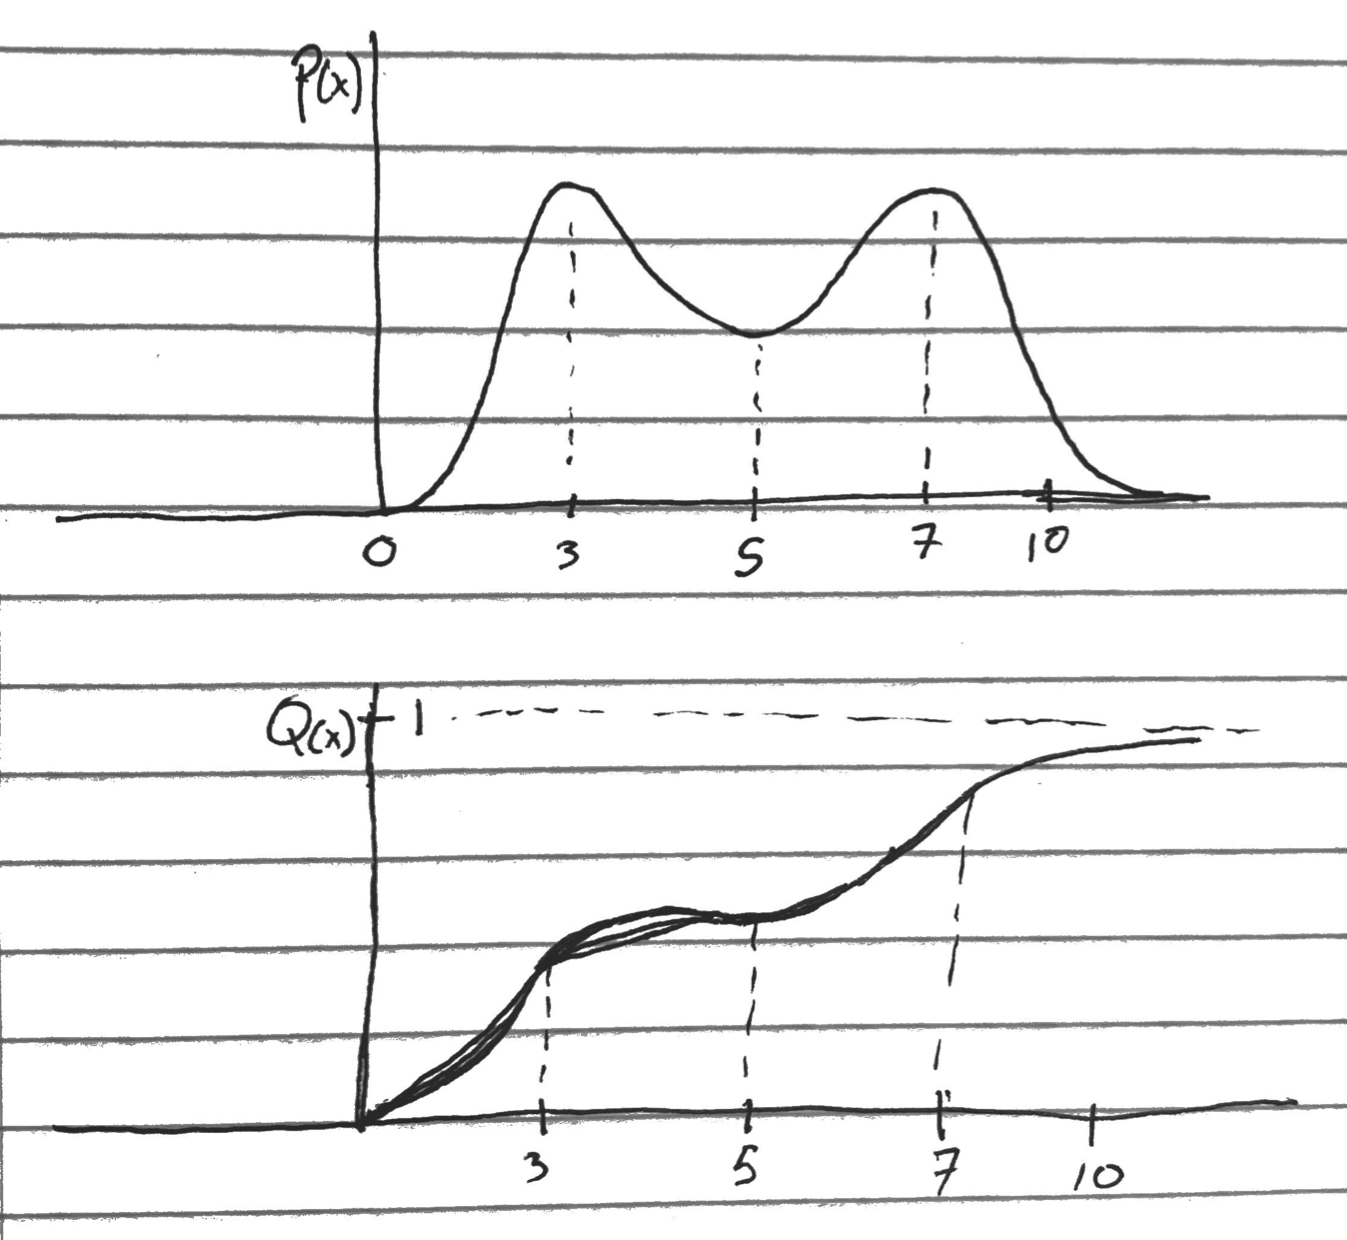
\includegraphics[width=\textwidth]{Midterm_Problem_1.png}
            \caption{Plots of an arbitrary $ p(x) $ and $ Q(x) $ for Problem 1.}
            \label{fig:problem_1_plot}
        \end{figure}
    \item[2.] Argue that if $ p(x) > 0 $ for all $ x $, the equation $ q = Q(x) $ can be solved for $ x = Q^{-1}(q) $ (meaning $ Q(x) $ is invertible).
        \begin{problem}
            An function is only invertible iff it is strictly increasing or decreasing in its domain. This corresponds to its derivative being strictly positive or negative over the entire domain. The probability distribution itself is the derivative of the cumulative distribution function by definition:
            \begin{equation}
                p(x) = \dv{Q(x)}{x}
            \end{equation}
            so as long as $ p(x) = \dv{Q(x)}{x} > 0 $ (or strictly negative), $ Q(x) $ is invertible.
        \end{problem}
    \item[3.] What is the domain over which the function $ Q^{-1}(q) $ is defined?
        \begin{problem}
            The CDF will increase from $ Q(- \infty) \equiv 0 $ to $ Q(\infty) \equiv 1 $ by definition, since $ \int_{a}^{a} f(x) \dd{x} \equiv 0 $ and $ \int_{- \infty}^{\infty} p(x) \dd{x} \equiv 1 $ if we require the probability distribution to be normalized (we do). Therefore, the domain of $ Q^{-1}(q) $ is $ q \in [0,1] $, since those are the maximum and minimum values obtainable from the CDF iff $ p(x) > 0 $.
        \end{problem}
    \item[4.] Let $ q $ be a random number chosen from the interval $ [0,1] $ with equal probability. Now prove the following statement, which is both interesting and practically useful: The random variable $ X := Q^{-1}(q) $ has the probability density $ p(x) $.

        Hint: $ X $ certainly has some probability density, let's call it $ p_{X}(x) $. Calculate it and discover that it coincides with $ p(x) $.
        \begin{problem}
            By transformation theory,
            \begin{equation}
                p_X(x') = \int_0^1 \dd{q} \delta(x' - Q^{-1}(q)) U(q)
            \end{equation}
            where $ U(q) $ is the uniform distribution and is equal to $ 1 $ in this domain. However, $ Q^{-1}(q) \equiv x $ sampled from $ p(x) $, so the $\delta$ function sets these distributions to be equal to each other.
        \end{problem}
    \item[5.] As an example: If someone can give you random numbers evenly distributed on $ [0,1] $, how would you create random numbers that are distributed according to the Cauchy-Lorentz density $ p_{x_0, a}(x) $ from problem 9 on homework sheet 3?
        \begin{problem}
            As seen in the previous problem, we just need to feed these numbers into the inverse CDF function for the Cauchy-Lorentz distribution:
            \begin{equation}
                p_{x_0, a}(x) = x_0 + a \tan(\pi \left(U(x) - \frac{1}{2}\right))
            \end{equation}
            where $ U(x) $ is, again, the uniform distribution for $ x \in [0,1] $.
        \end{problem}
\end{itemize}

\section*{2. Entropy of a Discrete Gas and its Legendre Transformation}
Consider a lattice with $ M $ sites, each of which can be either occupied by a particle or empty. Let's assume that exactly $ N $ sites are occupied. Don't worry about interactions\textemdash we assume they vanish. This is like an ideal gas on a lattice.
\begin{itemize}
    \item[1.] Calculate the total number $ \Omega(N,M) $ of of ways in which $ N $ sites on this lattice can be singly occupied.
        \begin{problem}
            The gas particles are not distinguishable in any way, so imagine we define an ordered set $ A = \{1,2,3, \cdots, M\} $. The number of ways we can fill lattice sites are the number of unique subsets of $ A $ which contain $ N $ elements, since we could imagine one such configuration of particles as choosing spots in $ A $ and adding those numbers to a new set until that set had $ N $ elements. I don't idly use the word ``choose'' here; This is a statement of ``$ M $ choose $ N $'', the definition of the binomial coefficient:
            \begin{equation}
                \Omega(N, M) = \binom{M}{N} = \frac{M!}{N!(M-N)!}
            \end{equation}
            The binomial coefficient $ \binom{M}{N} $ is defined as the number of ways to choose an unordered subset of $ N $ elements from a fixed set of $ M $ elements. We want this to be unordered choice because the particles are identical, and we don't want to double count all the different ways we could swap particles on the same lattice sites.
        \end{problem}
    \item[2.] The total entropy is given by $ S(N,M) = k_B \ln[\Omega(N,M)] $. Find an approximate expression for the entropy using the simplest version of Stirling's approximation.
        \begin{problem}
            \begin{align}
                S(N, M) &= k_B \ln[\Omega(N,M)] \\
                &= k_B \ln\left[\frac{M!}{N!(M-N)!}\right] \\
                &= k_B \left[ \ln M! - \ln N! - \ln(M-N)! \right]
            \end{align}
            Stirling's approximation states that, for $ n >> 1 $,
            \begin{equation}
                \ln n! = n\ln n - n + \order{\ln n} 
            \end{equation}
            Therefore,
            \begin{align}
                S(N,M) &\approx k_B \left[ M \ln M - M - N \ln N + N - (M - N) \ln (M - N) + M - N \right] \\
                &\approx k_B \left[ M \ln M - N \ln N - (M-N) \ln (M-N)\right] \\
                &\approx k_B \left[ M \ln\left( \frac{M}{M-N} \right) - N \ln\left( \frac{N}{M-N} \right)\right]
            \end{align}
        \end{problem}
    \item[3.] Define the fraction $ N/M =: \phi \in [0,1] $ of the occupied sites and express the entropy as $ S(\phi, M) $ or $ \tilde{s}(\phi) = S(\phi, M) / (M k_B) $.
        \begin{problem}
            $ \phi \equiv \frac{N}{M} \implies N = M \phi $, so
            \begin{align}
                S(\phi, M) &= k_B \left[ M \ln\left( \frac{M}{M - \phi M} \right) - \phi M \ln\left( \frac{\phi M}{M - \phi M} \right) \right] \\
                &= k_B M \left[ \ln\left( \frac{1}{1 - \phi} \right) - \phi\ln\left( \frac{\phi}{1-\phi} \right)\right] \\
                &= k_B M \left[ -\ln(1-\phi) - \phi\ln\phi + \phi\ln(1-\phi)\right] \\
                &= k_B M \left[ (\phi - 1)\ln(1 - \phi) - \phi\ln\phi\right]
            \end{align}
            or
            \begin{equation}
                \tilde{s}(\phi) = (\phi - 1)\ln(1 - \phi) - \phi\ln\phi
            \end{equation}
        \end{problem}
    \item[4.] Show that
        \subitem[(i)] $ S(\phi, M) = S(1 - \phi, M) $ and state in words what this means.
        \begin{problem}
            To avoid writing $ k_B $ and $ M $ a few times, I'll show equivalently that $ \tilde{s}(\phi) = \tilde{s}(1-\phi) $:
            \begin{align}
                \tilde{s}(\color{red}1-\phi\color{black}) &= (\color{red}(1-\phi)\color{black} - 1 ) \ln(1 -\color{red} (1-\phi)\color{black}) - \color{red}(1-\phi)\color{black}\ln\color{red}(1-\phi)\color{black}\\
                &= -\phi\ln\phi + (\phi - 1)\ln(1-\phi) \\
                &= \tilde{s}(\phi)
            \end{align}
            This is true because we could, at the beginning of the problem, have chosen $ M - N $ spaces to \textit{not} be occupied by gas particles. This would of course give the same binomial coefficient, but in terms of entropy, we could think of the vacant lattice sites in a particular microstate as being filled and vice-versa, and the entropy of the configuration shouldn't change (since we don't associate any intrinsic entropy with a gas particle existing and there are no interaction effects). $ \phi $ is just the filling fraction for the original case and $ 1-\phi $ is the filling fraction if we swap the identities of vacancies and particles, which does not change the number of possible microstates of the system $ \Omega $.
        \end{problem}
        \subitem[(ii)] The derivative $ \pdv{S}{\phi} $ can take any real number over the domain on which $ S(\phi, M) $ is defined.
        \begin{problem}
            \begin{align}
                \pdv{S}{\phi} &=  \pdv{\phi} \left[ k_B M \left[ (\phi - 1)\ln(1-\phi) - \phi\ln\phi \right] \right]\\
                &= k_B M \left( \left[ \ln(1-\phi) - \frac{\phi-1}{1-\phi} \right] - \left[ 1 + \ln\phi \right] \right)\\
                &= k_B M \left( \ln(1-\phi) - \ln\phi \right)\\
            \end{align}
            \begin{equation}
                \pdv{S}{\phi} \to \infty \qq{as} \phi \to 0
            \end{equation}
            and
            \begin{equation}
                \pdv{S}{\phi} \to - \infty \qq{as} \phi \to 1
            \end{equation}
            By the intermediate value theorem, $ \pdv{S}{\phi} $ must therefore take every value in $ (- \infty, \infty) $ at some point for $ \phi \in [0, 1] $.
        \end{problem}
        \subitem[(iii)] $ S(\phi, M) $ is concave in $ \phi $. Now plot it (as a function of $ \phi $).
        \begin{problem}
            To show concavity, I will take the second derivative with respect to $ \phi $:
            \begin{align}
                \pdv[2]{S}{\phi} &= \pdv{\phi} k_B M \left( \ln(1-\phi) - \ln\phi \right) \\
                &= - k_B M \left( \frac{1}{1-\phi} + \frac{1}{\phi}  \right)\\
                &= \frac{k_B M}{\phi(\phi - 1)}
            \end{align}
            In the domain of $ \phi $, this will always be negative because $ \phi - 1 $ will be negative for $ \phi < 1 $. Therefore, the function must be concave.
            
            See \Cref{fig:problem_2_4} for the plot of $ S(\phi, M) $. As predicted, the function is concave and symmetric about $ \phi = \frac{1}{2} $, the point with maximal entropy. The entropy expectedly decreases to zero at either end, where the gas either fully occupies the lattice or there is no gas at all.
        \end{problem}
        \begin{figure}[h]
            \centering
            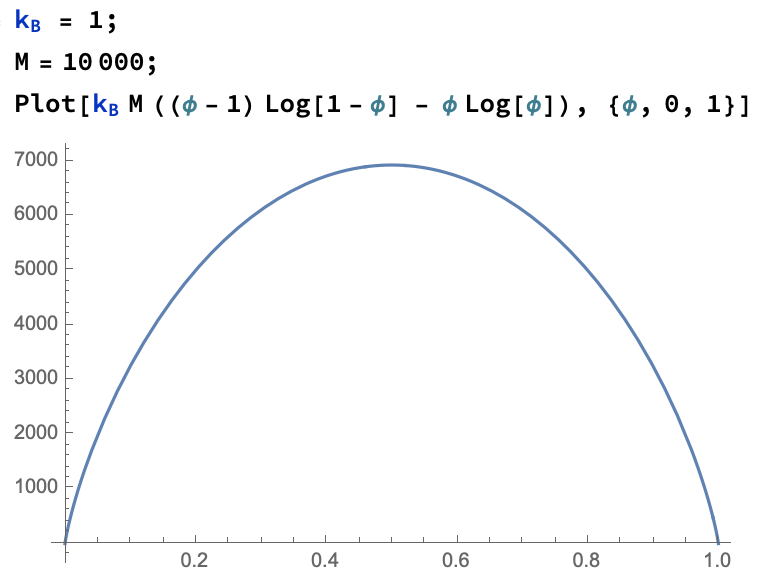
\includegraphics[width=\textwidth]{Midterm_Problem_2_Part_4.png}
            \caption{Plot for Problem 2 Part 4}
            \label{fig:problem_2_4}
        \end{figure}
    \item[5.] Define $ S^*(p, M) $ as the Legendre transform of $ S(\phi, M) $ with respect to $ \phi $ and calculate it. Plot it (as a function of $ p $).
        \begin{problem}
            We must maximize $ S(\phi, M) - \phi p $. We already know the derivative of $ S $, so we must now solve
            \begin{equation}
                k_B M \left( \ln(1-\phi) - \ln\phi \right) - p = 0
            \end{equation}
            in terms of $ \phi $:
            \begin{align}
                \ln\left( \frac{1-\phi_0}{\phi_0} \right) &= \frac{p}{k_B M} \\
                \frac{1-\phi_0}{\phi_0} &= e^{\frac{p}{k_B M}} \\
                &\implies \phi_0 = \frac{1}{1 + e^{\frac{p}{k_B M}}}
            \end{align}
            We then insert this back into the original maximization problem:
            \begin{align}
                S^*(p, M) &= \max_{\phi}(S(\phi,M) - p\phi) \\
                &= S(\phi_0, M) - p\phi_0 \\
                &= k_B M \left( (\phi_0 - 1)\ln(1-\phi_0) - \phi_0 \ln\phi_0 \right) - p \phi_0 \\
                &= k_B M \left( \frac{1}{1 + e^{\frac{p}{k_B M}}} - 1 \right) \ln\left( 1 - \frac{1}{1 + e^{\frac{p}{k_B M}}} \right) \\
                &- \left( \frac{1}{1 + e^{\frac{p}{k_B M}}}\right) \ln\left( \frac{1}{1 + e^{\frac{p}{k_B M}}} \right) - \frac{p}{1 + e^{\frac{p}{k_B M}}} \\
                &= k_B M \left(-\frac{\ln \left(\frac{1}{e^{\frac{p}{k_B M}}+1}\right)}{e^{\frac{p}{k_B M}}+1}-\frac{e^{\frac{p}{k_B M}}}{e^{\frac{p}{k_B M}}+1} \ln \left(\frac{e^{\frac{p}{k_B M}}}{e^{\frac{p}{k_B M}}+1}\right)\right)-\frac{p}{e^{\frac{p}{k_B M}}+1} \\
                &= k_B M \left(\frac{\ln \left(e^{\frac{p}{k_B M}}+1\right)}{e^{\frac{p}{k_B M}}+1}-\frac{e^{\frac{p}{k_B M}}}{e^{\frac{p}{k_B M}}+1} \left(\ln \left(e^{\frac{p}{k_B M}}\right)-\ln \left(e^{\frac{p}{k_B M}}+1\right)\right)\right)-\frac{p}{e^{\frac{p}{k_B M}}+1}\\
                &= k_B M \left(\ln \left(e^{\frac{p}{k_B M}}+1\right)-\frac{e^{\frac{p}{k_B M}}}{e^{\frac{p}{k_B M}}+1}\ln \left(e^{\frac{p}{k_B M}}\right)\right)-\frac{p}{e^{\frac{p}{k_B M}}+1} \\
                &= k_B M \left(\ln \left(e^{\frac{p}{k_B M}}+1\right)- \frac{e^{\frac{p}{k_B M}}}{e^{\frac{p}{k_B M}}+1}\frac{p}{k_B M}\right)-\frac{p}{e^{\frac{p}{k_B M}}+1} \\
                S^*(p, M) &= k_B M \ln \left(e^{\frac{p}{k_B M}}+1\right)-p
            \end{align}
            See \Cref{fig:problem_2_5} for a plot of $ S^*(p, M) $ as well as the Mathematica code used to produce it. I set $ k_B = 1 $ since it's just an arbitrary scale factor to get units of entropy, and $ M = 10000 $ as an arbitrary large lattice size.
        \end{problem}
        \begin{figure}[h]
            \centering
            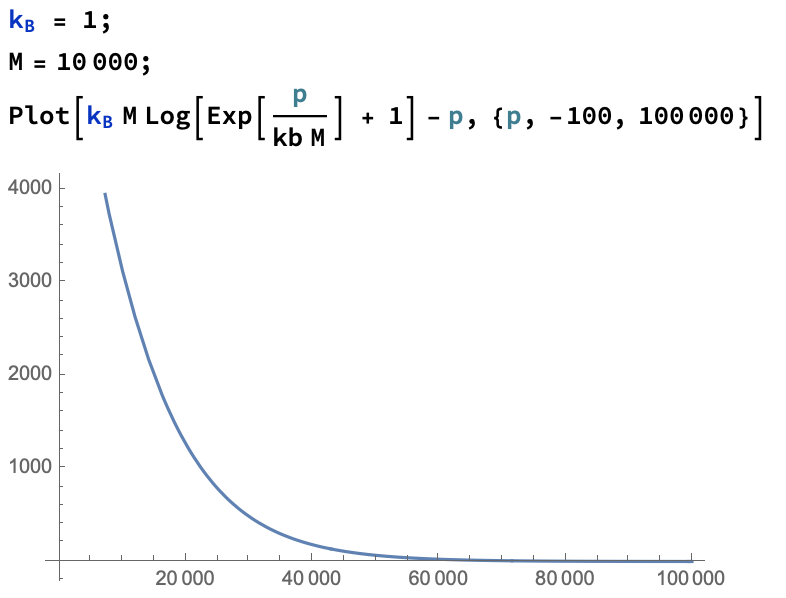
\includegraphics[width=\textwidth]{Midterm_Problem_2_Part_5.png}
            \caption{Plot for Problem 2 Part 5}
            \label{fig:problem_2_5}
        \end{figure}
\end{itemize}

\section*{3. Generalized Harmonic/Arithmetic Mean Inequality}
Consider $ N $ positive numbers $ x_i $, associated with the weights $ p_i $, which satisfy $ 0 \leq p_i \leq 1 $ and $ \sum_{i=1}^{N} p_i = 1 $. Prove the following inequality between the generalized harmonic and the generalized arithmetic mean:
\begin{equation}
    \left( \sum_{i=1}^{N} p_i \frac{1}{x_i} \right)^{-1} =: \ev{\{x_i\}}_{\text{GH}} \leq \ev{\{x_i\}}_{\text{GA}} := \sum_{i=1}^{N} p_i x_i.
\end{equation}
\begin{problem}
    By the Cauchy-Schwartz Inequality,
    \begin{align}
        \sum_{i=1}^{N} \frac{p_i}{x_i} \sum_{i=1}^{N} p_i x_i &\geq \left( \sum_{i=1}^{N} \sqrt{\frac{p_i}{x_i}} \sqrt{p_i x_i} \right)^2 \\
        &= \left( \sum_{i=1}^{N} \sqrt{p_i^2} \right)^2 \\
        &= \left( \sum_{i=1}^{N} p_i \right)^2 \\
        &= 1^2 = 1
        \implies 1 \leq \frac{\ev{\{x_i\}}_{\text{GA}}}{\ev{\{x_i\}}_{\text{GH}}} \implies \ev{\{x_i\}}_{\text{GH}} \leq \ev{\{x_i\}}_{\text{GA}}
    \end{align}
\end{problem}


\section*{4. One of them Thermodynamic Identities\ldots}
Rewrite the following partial derivative in terms of the usual response functions (meaning: thermal expansion coefficient, either one of the compressibilities, either one of the specific heats), and of course any of the other functions of state, such as $ T $, $ S $, $ P $, $ V $, \ldots, and possibly innocent numbers:
\begin{equation}
    \eval{\pdv{U}{P}}_{G,N} = ?
\end{equation}

Hints:
\begin{itemize}
    \item[(1)] The thermodynamic potential $ G(T, P, N) $ is the Gibbs free energy.
    \item[(2)] The answer will not look particularly pretty. Don't worry about this\textemdash it's not your fault. Instead, take pride in your thermodynamic superpowers that enable you to derive results like this.
    \item[(3)] The standard Jacobi expansion is a good way to start, even if one of the new Jacobians cannot be reverse-Jacobified; Handle that obdurate one by dealing with it as an actual determinant. From then on, you can go on auto-pilot.
\end{itemize}

\begin{problem}
    \begin{align}
        \eval{\pdv{U}{P}}_{G,N} &= \pdv{(U,G)}{(P,G)} \\
        &= \pdv{(U,G)}{(P,T)} \underbrace{\pdv{(P,T)}{(P,G)}}_{- \frac{1}{S}} \\
        &= - \frac{1}{S} \left[ \overbrace{\eval{\pdv{U}{P}}_{T}}^{\ast} \underbrace{\eval{\pdv{G}{T}}_{P}}_{-S} - \underbrace{\eval{\pdv{G}{P}}_{T}}_{V} \overbrace{\eval{\pdv{U}{T}}_{P}}^{\dagger} \right] \\
    \end{align}
    \begin{align}
        \ast &= \eval{\pdv{U}{P}}_{T} \\
        &= T \eval{\pdv{S}{P}}_{T} - P\underbrace{\eval{\pdv{V}{P}}_{T}}_{- \kappa_T V} \\
        &= - T \underbrace{\eval{\pdv{V}{T}}_{P}}_{\alpha V} + P\kappa_T V \\
        &= PV \kappa_T - \alpha TV
    \end{align}
    \begin{align}
        \dagger &= \eval{\pdv{U}{T}}_{P} \\
        &= T \underbrace{\eval{\pdv{S}{T}}_{P}}_{\frac{C_P N}{T}} - P \underbrace{\eval{\pdv{V}{T}}_{P}}_{\alpha V} \\
        &= C_P N - PV \alpha
    \end{align}

    Therefore
    \begin{align}
        \eval{\pdv{U}{P}}_{G,N} &= - \frac{1}{S} \left( -S(PV \kappa_T - \alpha TV) - V(C_P N - PV \alpha) \right) \\
        &= PV \kappa_T - TV \alpha + \frac{VC_P N}{S} - \frac{PV^2 \alpha}{S}
    \end{align}
\end{problem}











\end{document}
